\documentclass[12pt, a4paper]{report}
\usepackage[utf8]{inputenc}

% hyperref
\usepackage[bookmarks, colorlinks, breaklinks]{hyperref}  % PDF hyperlinks, with coloured links
\hypersetup{linkcolor=black, citecolor=black, filecolor=black, urlcolor=black} % black links, for printed output

% Support for the inclusion of figures
\usepackage{graphicx}

% "Contents" and "bibliography" are included in the summary.
\usepackage{tocbibind}

% Packages and configuration for Alloy code listing
%\usepackage{listings}
%\usepackage{alloy}
%\usepackage{color}
%\definecolor{alloy-keyword}{rgb}{0.23, 0.23, 0.7}
%\definecolor{alloy-comment}{rgb}{0.18, 0.64, 0.18}
%\definecolor{alloy-string}{rgb}{0.71, 0.18, 0.71}

\def\chapterautorefname{Chapter}

\begin{document}
\title{Software Engineering 2: TrackMe \\ \vspace{1em} Requirements Analysis and Specification Document}
\author{Haritha Harikumar, Mohini Gupta, Saloni Kyal\\
Politecnico di Milano}
\date{November 11, 2018}
\maketitle
\tableofcontents

%%%%%% INTRODUCTION %%%%%%%%
\chapter{Introduction}
\label{ch:introduction}

\section{Purpose}
The document represents the Requirement Analysis and Specification Document for the application named TrackMe. TrackMe is an web/android application that provides a certain services like vital monitoring, emergency services for elderly people and real time visualization of race or marathons. 

This document focuses to completely describe the TrackMe system in terms of functional and non-functional requirements, analyze the real needs of the customer in order to model the system. We also focus on the constraints and the limitations of the software to indicate the typical use cases. 

Further, this document will provide formal specification of some features of the applications, by means of the Alloy language~\cite{alloy-site}.

The document is addressed to both the customers which specifies the requirements as mentioned by the customers and the developers who have to implement the requirements.

\section{Scope}
The system is a taxi reservation and dispatching system for large cities. Its main goal is to simplify the access of passengers to the service and to guarantee a fair management of taxi queues.

The system consists in a back-end server application (\emph{myTaxi Server}), a web application front-end (\emph{myTaxi Web}) and in a mobile application (\emph{myTaxi Mobile}).

The system has 2 types of users: passengers and taxi drivers; it should allow the users to sign up and login with their credentials.
The system has to know the location of both the passengers and the taxi drivers.

The system allows any passenger to request a taxi, informing him or her about the incoming taxi code and the estimated waiting time.

The system knows about the available taxi drivers and, when a request is incoming, informs one of them about the location of the available passenger; the taxi driver can either accept or deny the ride.
If the taxi driver accepts the ride, the system sends a confirmation to the passenger, together with the estimated waiting time.
If the taxi driver rejects the ride, the system looks for another taxi driver in the same area of the city.

The system offers programmatic interfaces (APIs) to enable the development of additional services on top of the basic one.



\section{Goals}
\subsection{Goals}
\begin{itemize}
\item \textbf{G1} Providing a list of the wearable devices that an individual can choose from.
\item \textbf{G2} Get a permission from an individual to access their health and location details from the wearable device.
\item \textbf{G3} Expedite the request made by the 3rd party to an individual to access their details.
\item \textbf{G4} Provides an interface for an individual to analyse the request made by the 3rd party.
\item \textbf{G5} Validating the request made by the 3rd party to provide the details of a group of individuals.
\item \textbf{G6} Quick access of the data to the 3rd party once the request is approved.
\item \textbf{G7} Immediate update of the data once an individual updates their own details.
\item \textbf{G8} Provides an upgradation to the new services, Automated SOS or Track4Run.
\item \textbf{G9} Monitoring the health status of the subscribed individual to the Automated SOS service.
\begin{itemize}
\item \textbf{G9.1} Alerts the nearby ambulance, when the health status of the individual is low, within 5 seconds.
\end{itemize}
\item \textbf{G10} Develops an interface to organize a race for the subscribed 3rd party to the Track4Run service.
\item \textbf{G11} Give access to the details of the race once an individual participate in it.
\item \textbf{G12} Provides a map interface to view the race live.
\end{itemize}




\section{Definitions, acronyms, and abbreviations}
\subsection{Definitions}
\begin{enumerate}
\item Services: Functionalities offered by the application
\item Validation: Verifying if requests provided by the 3rd party are genuine or not. If it is genuine it is accepted else rejected.
\item Upgrade: Enhancing the functionalities. 
\item Update: Adding new information or changing the previous one.
\item Threshold: A limit. Threshold on age has been kept for Automated SOS service.
\item Push Notification: The message that pops up on the Mobile. 
\end{enumerate}

\subsection{Acronyms}
\begin{enumerate}
\item RASD: Requirement Analysis and Specification Document
\item API: Application Program Interface
\item GPS: Global Positioning System
\item SOS: Save our Souls
\end{enumerate}

\subsection{Abbreviations}
\begin{enumerate}
\item Gn: n-Goal
\item An: n-Assumption
\item Dn: n-Dependency
\item Cn: n-Constraint
\item Rn: n-Functional Requirement 
\end{enumerate}


\section{References}
\begin{itemize}
\item Specification Document: "Mandatory Project Assignment AY 2018-2019.pdf"
\item Alloy model example: "http://alloytools.org/tutorials/online/"
\item Requirement Engineering Slides I, II
\item Alloy Slides 
\end{itemize}

\section{Overview}
\qquad The RASD is composed of 6 parts including references
\begin{enumerate}
\item The first part is an introduction to the problem which identifies the scope and goals of the application to be developed. Apart from this different definitions, acronyms and abbreviations used in the document are also noted down here.
\item The second part of the document comprises of the overall description of the application which includes product functionalities, the users involved and the assumptions, dependencies and constraints.
\item The third part of the document takes into the specific requirements like the interfaces used, functional requirements and the different unified modeling language diagrams and the non-functional requirements.
\item The fourth part of the document is the Alloy code and metamodel we have created.
\item The fifth part of the document is the effort spend by each of the Team Members
\item The last part of the document has all the references
\end{enumerate}

%%%%%% OVERALL DESCRIPTION %%%%%%%%
\chapter{Overall description}
\label{ch:overall-desc}

%\section{Product perspective}
%\subsection{Class Diagram}
\begin{figure}[H]
	\begin{center}	
		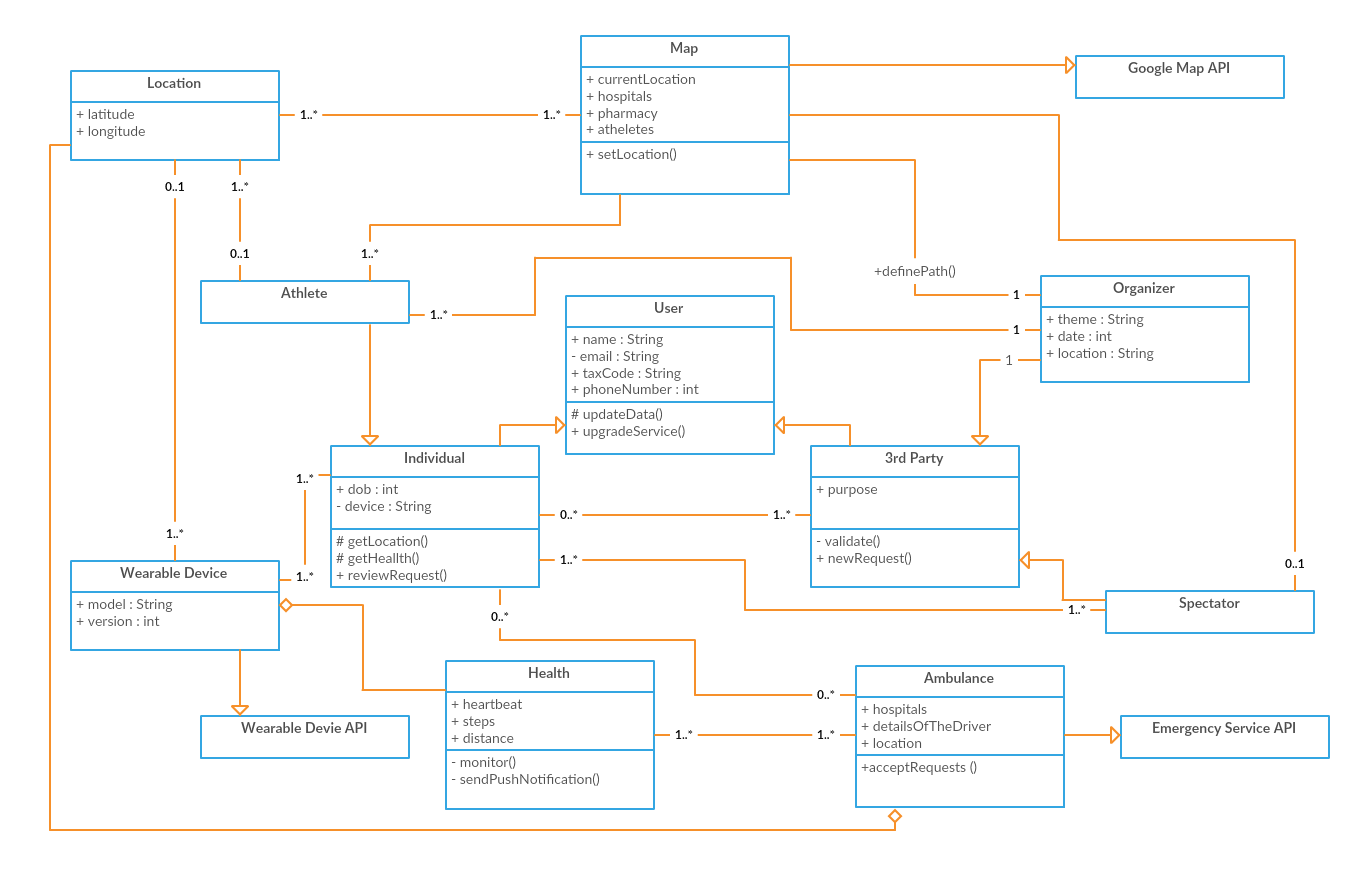
\includegraphics[width=\textwidth]{./Diagrams/ClassDiagram.png}
      	\caption{Class Diagram for TrackMe}
        \label{TrackMe_classdiagram}
	\end{center}
\end{figure}

%---------------STATE DIAGRAM----------------------%
\subsection{State Charts}
\begin{figure}[H]
	\begin{center}
		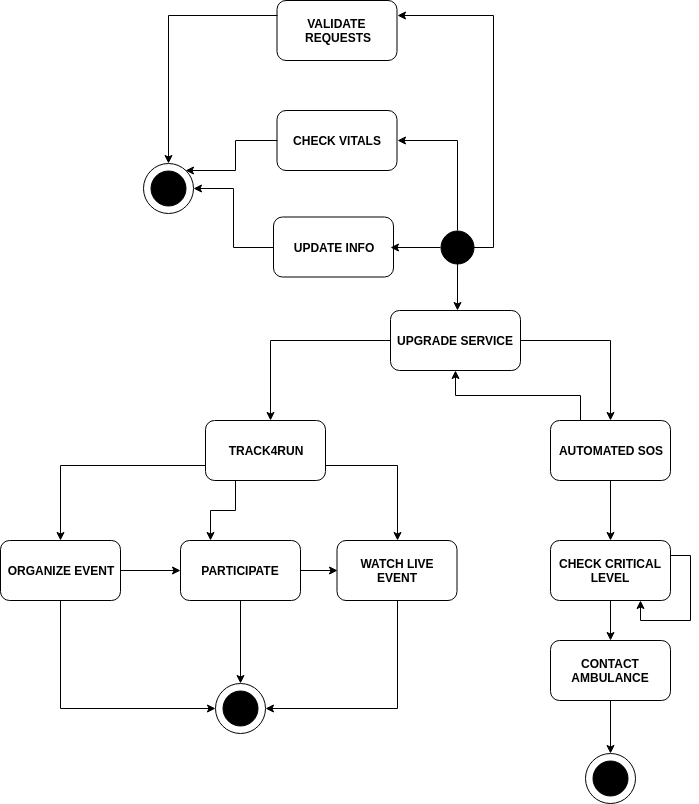
\includegraphics[width=\textwidth]{./Diagrams/StateDiagram.png}
      	\caption{State Diagram for TrackMe}
        \label{TrackMe_statediagram}
	\end{center}
\end{figure}

\section{Product functions}
\subsection{Vital Status}

% to be added

\subsection{Location Tracking}
\qquad Data4Help helps TrackMe to use monitor the location of the individual which can be later shared with the third party after validation. This service of location tracking can be helpful in case of emergencies which we come across in automated SOS. We basically use the Global Positioning System or the GPS to track the location of the individual. There are chances that we can lose the GPS connection in certain cases like may be inside our home due to poor connection to satellite. In such cases we can fetch the location from the nearest wi-fi to which our device get connected. In case of an emergency TrackMe system shall locate a minimum of 3 available ambulances that are closest to the emergency location by displaying a map and marking location of the emergency and ambulance nearby, which is would be taking less than a minute to fetch. We then share the data to the nearest ambulance within 5 seconds.We also use location tracking for athletes for a real time visualization of the positions of the athletes for a particular race which is explained further below.


\subsection{Third Party Validation}
% To be added

\subsection{Organizing a Race}
%to be added

\subsection{Expeditious Data Convey}
%to be added

\subsection{Real Time Visualization of Race}
\qquad This service is basically used by the spectators who wish to watch a race or marathon live, which comes as a part of the Track4Run. Once an athlete registers with the Track4Run service. His/Her location is tracked live with the help of the device using GPS. Track4Run fetches the track details way before and set it as the Track for a particular race or marathon and shows an enlarged view of the track while displaying the live positions of the participants.

\section{User characteristics}
\subsection{Individual}
A person using TrackMe for monitoring his/her vitals using the Data4Help service. He/She gets to register for the service by making an monthly payment and his/her data would be tracked and monitored by the TrackMe.
\subsection{Third Party} 
This can be a person or a company who wish to get the data for the users for some work of his/her concern. They have to register by making a certain payment amount as specified by TrackMe and a valid purpose for the data transfer. The transfer of data is based after proper analysis and validation by the TrackMe.
\subsection{Organizers}
Organizers are those people who use the Track4Run service, who wish to organize an event like a race or a marathon for a cause. They have to register the event with the details of the event, location, date, time and so on. Track4Run is a paid service and hence organizers have to register with a specific cost.
\subsection{Athletes} 
These are those people who join for a specific event organized by mentioning details like name, contact and wearable device to be used and complete the registration by making the payment.
\subsection{Spectators}
These are people who wish to avail the service of Track4Run just to watch the race. He/She can just join to watch a particular race by providing basic details like name, email and the one time payment amount. They can also upgrade their service to watch the upcoming events or receive notifications on upcoming races.
\subsection{Ambulance Drivers}
TrackMe has an application for the Ambulance drivers who gets push notifications from Automated SOS service.  


%\section{Constraints}
%\input{overall_description/constraints.tex}

%\section{Assumptions and dependencies}
%\subsection{Assumptions}
\begin{itemize}
\item \textbf{[A1]} Users should be registered in the TrackMe application to avail its services.
\item \textbf{[A2]} There exist a mobile application of TrackMe for individuals and third party.
\item \textbf{[A3]} Vitals taken from the wearable devices are reliable. 
\item \textbf{[A4]} Internet connection will be active in users phone. 
\item \textbf{[A5]} GPS provides accurate positions and in case the signal is lost, last active location would be considered.
\item \textbf{[A6]} We assume that a certain number of hospitals are registered to with TrackMe which provide Ambulance services.
\item \textbf{[A7]} We assume there are no network issues between the time we sent a message and the drivers receive it.
\item \textbf{[A8]} Organizers can keep a maximum limit of the participants who can join the event.
\item \textbf{[A9]} An event is organized for a reason.
\item \textbf{[A10]} All athletes have their own wearable device.
\item \textbf{[A11]} A user can be an individual or a third party. An individual can either belong to the people availing Data4Help or they can be spectator. An organizer belongs to the third party group. An athlete belongs to the individual group.
\item \textbf{[A12]} All details entered by the users are genuine.
\item \textbf{[A13]} We take permission from user to access the location and further details.
\item \textbf{[A14]} There is an external service that will be in charge of the payment information and to ensure secure payment.
\item \textbf{[A15]} Payment Details are genuine and transactions are processed positively.
\end{itemize}

\subsection{Dependencies}
\begin{itemize}
\item{\textbf{[D1]}} Wearable device API
\item{\textbf{[D2]}} Google Maps API
\item{\textbf{[D3]}} Emergency services API
\item{\textbf{[D4]}} Payment external gateway
\end{itemize}

\subsection{Constraints}
\begin{itemize}
\item{\textbf{[C1]}} Only a few wearable devices are compatible with application.
\item{\textbf{[C2]}} The services provided by the application are limited to the citizens of Milan.
\item{\textbf{[C3]}} This application is connected only with the major hospitals in Milan for Ambulance services.
\end{itemize}

%\section{Future extensions}
%\input{overall_description/extensions.tex}

%%%%%% SPECIFIC REQUIREMENTS %%%%%%%%
\chapter{Specific requirements}
\label{ch:requirements}

\section{External interface requirements}
\subsection{User Interfaces}


\subsection{Hardware Interfaces}


\subsection{Software Interfaces}
\begin{enumerate}
\item \textbf{Data4Help API}
\newline \qquad TrackMe extracts location and health of the individual from the API of the   wearable device and stores it in a database. An API of the database is created which is provided to the other services of TrackMe. This information is used for many purposes. “AutomatedSOS” and “Track4Run” uses the API of the “Data4Help” in order to provide their service. Both the services exploit the services of “Data4Help”. “AutomatedSOS” uses the API to monitor the health status of elderly people and help them by providing an ambulance. “Track4Run” uses the API to extract the location and health of individuals registered as athletes. The location will be displayed to all the users and the health status of athletes will be monitored by the third party organizers.
\item \textbf{Ambulance Application}
\newline\qquad TrackMe develops an application for all the ambulance drivers associated with major Hospitals in the city of Milan. The application fetches the details and location of all the ambulance driver. When the health status of an subscribed individual is below a threshold value, the software sends a push notification to the nearby ambulance drivers phone with the details and location of the individual. Once an ambulance driver accept the request, the software removes the alert message from the application. The driver can navigate to the location of the individual in need of emergency using the map provided in the application.
\item \textbf{City Maps}
\newline\qquad We will be using Google Maps API to facilitate the location monitoring for third party services and insertion of race location in Track4Run and race visualization.
\item \textbf{Communication Interfaces}
\end{enumerate}

%\section{System features}
%\input{specific_requirements/system_features.tex}

%\section{Performance requirements}
%\input{specific_requirements/performance.tex}

%\section{Software system attributes}
%\input{specific_requirements/software_system_attributes.tex}

%\section{Alloy}
%\subsection{Description}
To execute the main objective, the alloy model depicts the following logics:
\begin{itemize}
\item There are two users individual and third party.
\item Individual has one wearable device that gives Location and Health vitals of that Individual.
\item Third Party can make Group Request and Individual Request.
\item When the health status of an Individual is below the threshold value, the critical condition is True.
\item The ambulance gets the details of the individual whose critical condition is true.
\item The details of the individual is connected to the ambulance that is near to the individual location.
\item An organizer is a Third Party who organizes the Event.
\item An Athlete is an Individual who joins the Event.
\item A spectator can be both Individual and Third party who watches the event.
\item An event has date, time, and location.
\end{itemize}
\subsection{Alloy code}
\begin{figure}[H]
	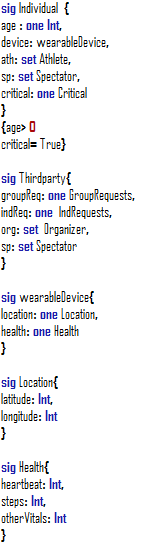
\includegraphics[width=5cm,height=18cm]{./Alloy/sig1.PNG}
\end{figure}
\begin{figure}[H]	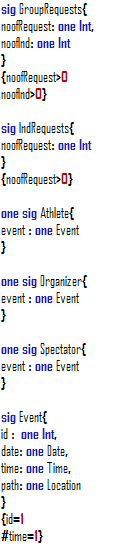
\includegraphics[width=5cm,height=18cm]{./Alloy/sig2.PNG}
\end{figure}
\begin{figure}[H]	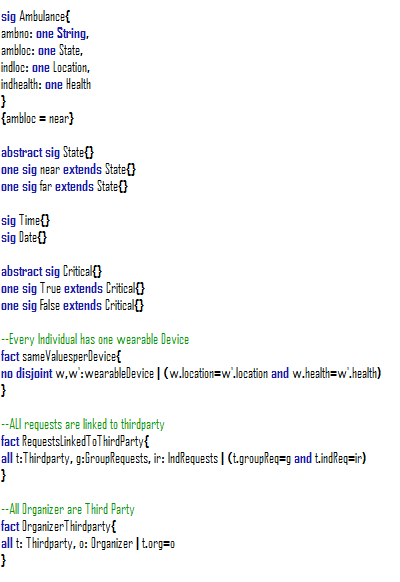
\includegraphics[width=\linewidth]{./Alloy/sig3+fact1.PNG}
\end{figure}
\begin{figure}[H]	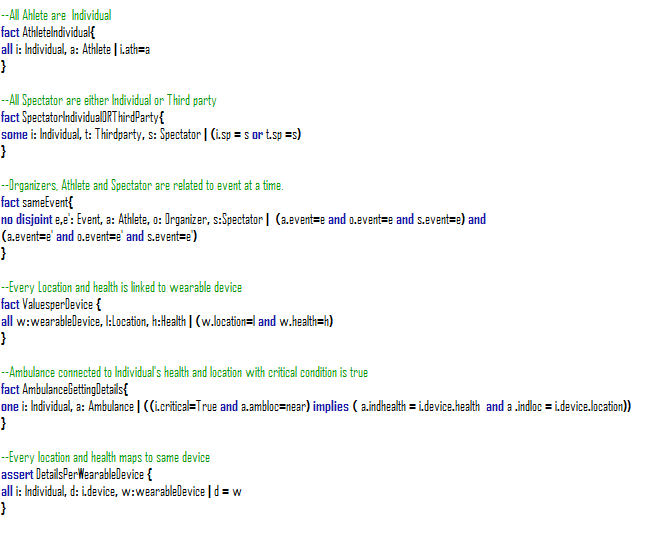
\includegraphics[width=16cm,height=18cm]{./Alloy/fact2+assert1.PNG}
\end{figure}
\begin{figure}[H]	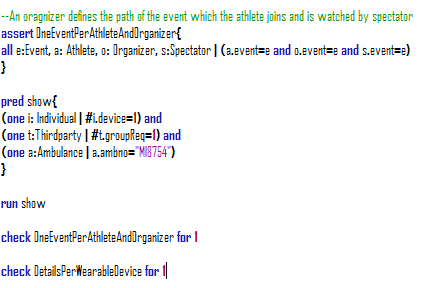
\includegraphics[width=16cm,height=12cm]{./Alloy/assert2+pred.PNG}
\end{figure}
\subsection{Result}
\begin{figure}[H]	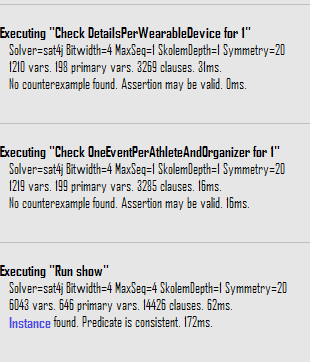
\includegraphics[width=\linewidth]{./Alloy/Result.PNG}
\end{figure}
\subsection{Alloy Model}
\begin{figure}[H]	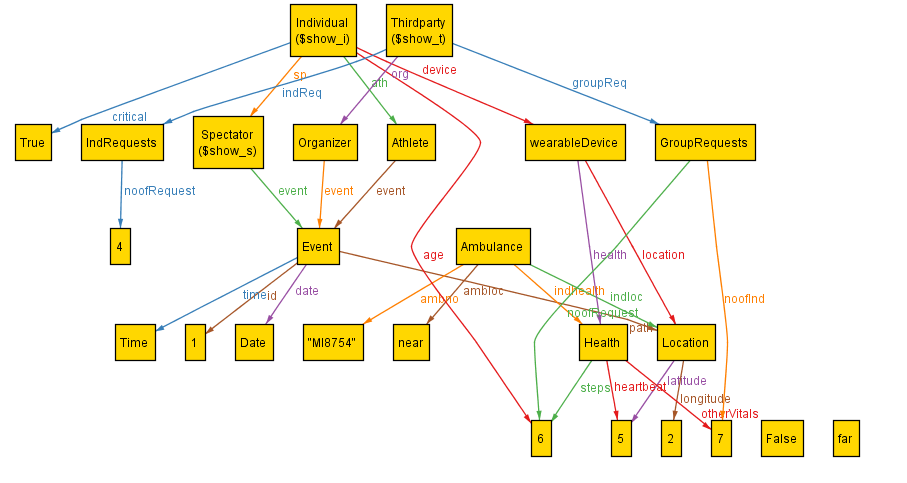
\includegraphics[width=\linewidth]{./Alloy/Final_model.PNG}
\end{figure}

%\appendix
%\chapter{Appendix}
%\input{appendix.tex}

%\input{bibilography.tex}

\end{document}